% Homework Template
\documentclass[UTF8, a4paper]{article}
\usepackage{ctex}
\usepackage{amsmath, amssymb, amsthm}
\usepackage{moreenum}
\usepackage{mathtools}
\usepackage{url}
\usepackage{bm}
\usepackage{enumitem}
\usepackage{graphicx}
\usepackage{subcaption}
\usepackage{booktabs} % toprule
\usepackage[mathcal]{eucal}
\usepackage[thehwcnt = 1]{iidef}

\thecourseinstitute{清华大学电子工程系}
\thecoursename{\textbf{媒体与认知} \space 课堂2}
\theterm{2021-2022学年春季学期}
\hwname{作业}
\begin{document}
\courseheader{test}
\name{李智毅}
\vspace{3mm}
\centerline{\textbf{\Large{理论部分}}}

\section{单选题(15分)}
\subsection{\underline{B}}

\subsection{\underline{C}}

\subsection{\underline{A}}

\subsection{\underline{B}}

\subsection{\underline{B}}

\section{计算题(15 分)}

\begin{figure}[h]
    \centering
    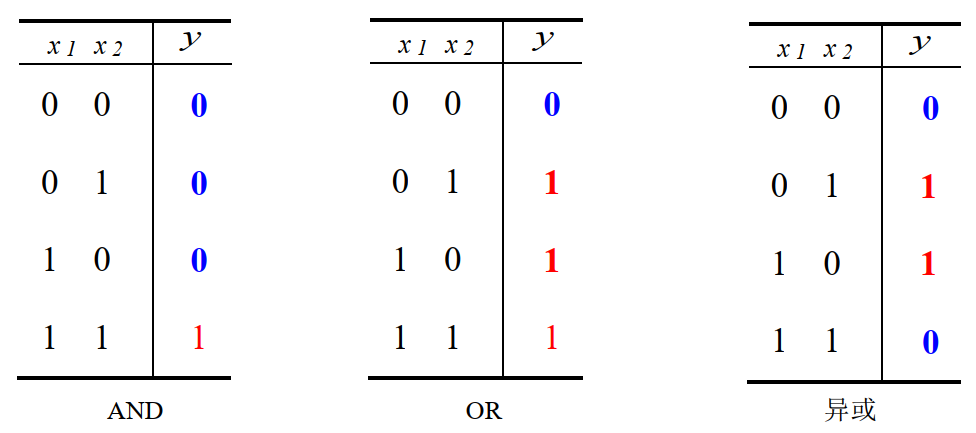
\includegraphics[width=12cm]{Fig1.png}
    \caption{AND,OR,异或三种逻辑运算}
    \label{fig:label_1}
\end{figure}

\subsection{基于如下单个人工神经元,设计实现两种逻辑门AND、OR运算。}
\begin{equation}
    z=w_1x_1 +w_2x_2 + b
\end{equation}
\begin{equation}
y=f(z)=\left\{
        \begin{array}{lr}
        1, z > 0 \\
        0, z \leq 0
        \end{array}
\right.
\end{equation}
\textbf{实现AND运算:}
取$ w_1=0.5 $,$ w_2=0.5 $,$ b=-0.75 $,因此有
\begin{center}
    \begin{tabular}{| c | c | c | c |}
        \hline
        $ x_1 $ & $ x_2 $ & $ z $ & $ y $ \\
        \hline
        0 & 0 & -0.75 & 0 \\
        1 & 0 & -0.25 & 0 \\
        0 & 1 & -0.25 & 0 \\
        1 & 1 & 0.25 & 1 \\
        \hline
    \end{tabular}
\end{center}
\textbf{实现OR运算:}
取$ w_1=0.5 $,$ w_2=0.5 $,$ b=-0.25 $,因此有
\begin{center}
    \begin{tabular}{| c | c | c | c |}
        \hline
        $ x_1 $ & $ x_2 $ & $ z $ & $ y $ \\
        \hline
        0 & 0 & -0.25 & 0 \\
        1 & 0 & 0.25 & 1 \\
        0 & 1 & 0.25 & 1 \\
        1 & 1 & 0.75 & 1 \\
        \hline
    \end{tabular}
\end{center}
\subsection{上述形式的单个神经元是否可以实现逻辑门异或运算?如果是,请给出具体设计;若否,请解释理由。}
不可以;\\
异或操作满足的逻辑运算如下:
\begin{center}
    \begin{tabular}{| c | c | c |}
        \hline
        $ x_1 $ & $ x_2 $ & $ y $ \\
        \hline
        0 & 0 & 0 \\
        1 & 0 & 1 \\
        0 & 1 & 1 \\
        1 & 1 & 0 \\
        \hline
    \end{tabular}
\end{center}
此时,需要分类的两种类别占据正方形的对角处,而题中所给出的单个人工神经元的感知机或逻辑回归模型的线性分类模型,相当于以一条直线\ $ y=kx+b $\ 对样本点进行切分,而异或操作不满足此要求,因此单个人工神经元不能解决二分类问题。\\

\vspace{6mm}
\centerline{\textbf{\Large{编程部分}}}
\vspace{3mm}
% 请根据是否选择自选课题的情况选择“编程作业报告”或“自选课题开题报告”中的一项完成
\section{编程作业报告}
按照题目要求,可以设计模型并运行如下。
\subsection{模型建立与代码撰写}
\subsubsection{定义数据类模块}
主要内容是完成文件读取、(内置)求长函数及下标函数。\\
文件读取:分别建立self.features和self.labels以存放特征与标签。\\
求长函数:返回self.features的第一个维度信息即可。\\
下标函数:需要判断是否越界,在合理范围内即返回相应下标的信息。
\subsubsection{定义模型结构}
需要完成模型初始化与前向传播函数。\\
模型初始化:定义单层网络模型,即构造self.weight与self.bias,其规模由输入数据规模决定;同时定义线性传播与激活函数,激活函数选择Sigmoid函数。\\
前向传播函数:对于每一个x依次通过线性层与非线性激活层,返回输出结果。
\subsubsection{定义损失函数}
根据交叉熵定义,求相应交叉熵即可。
\subsubsection{训练-验证代码}
需要完成对象的实例化、每轮的训练过程以及验证过程。\\
对象实例化:实例化网络、数据集、优化器等。\\
训练过程:包括前向计算、反向传播、loss计算、梯度计算等步骤。\\
验证过程:将数据通过网络,输出与label进行比较。

\subsection{训练、测试、可视化}
\subsubsection{训练过程}
训练模型,运行\ python classification.py train\ ,得到以下loss曲线(见图2)。\\
\begin{figure}
    \centering
    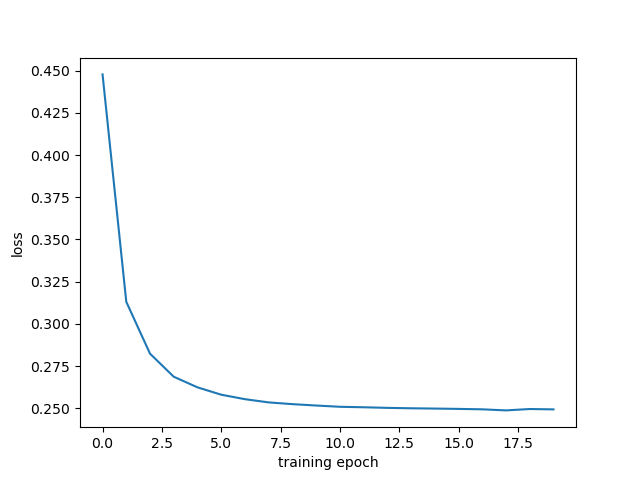
\includegraphics[width=12cm]{Fig2.png}
    \caption{训练过程的loss曲线}
\end{figure}
可以看到,在训练过程中,网络模型收敛速度很快,在3轮后基本稳定,验证准确率达90\%以上。训练完成后,保存模型。\\
测试模型,运行\ python classification.py test\ ,得到测试集准确率90.6\%。\\
可视化,运行\ python classification.py visual\ ,得到可视化结果(见图3)。
\begin{figure}
    \centering
    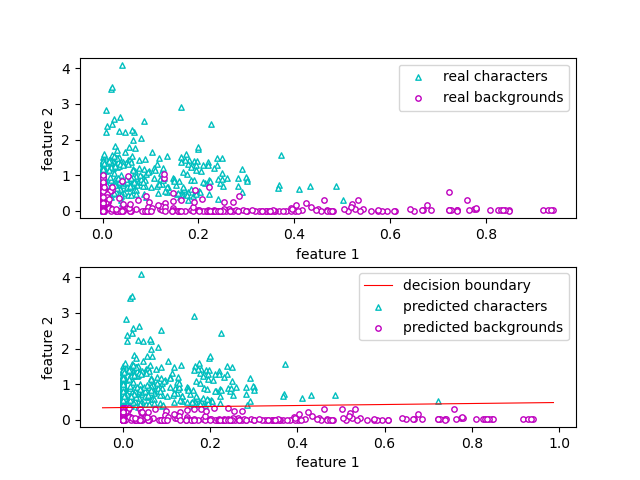
\includegraphics[width=12cm]{Fig3.png}
    \caption{模型的线性决策面}
\end{figure}

\end{document}



%%% Local Variables:
%%% mode: late\rvx
%%% TeX-master: t
%%% End:
